\subsection{Ερώτημα iv}
   \begin{minipage}{\textwidth}
      \begin{center}
         \fbox{\textlatin{\textbf{\textit{Kaby Lake Microarchitecture}}}}\\
         \vspace{3mm}
         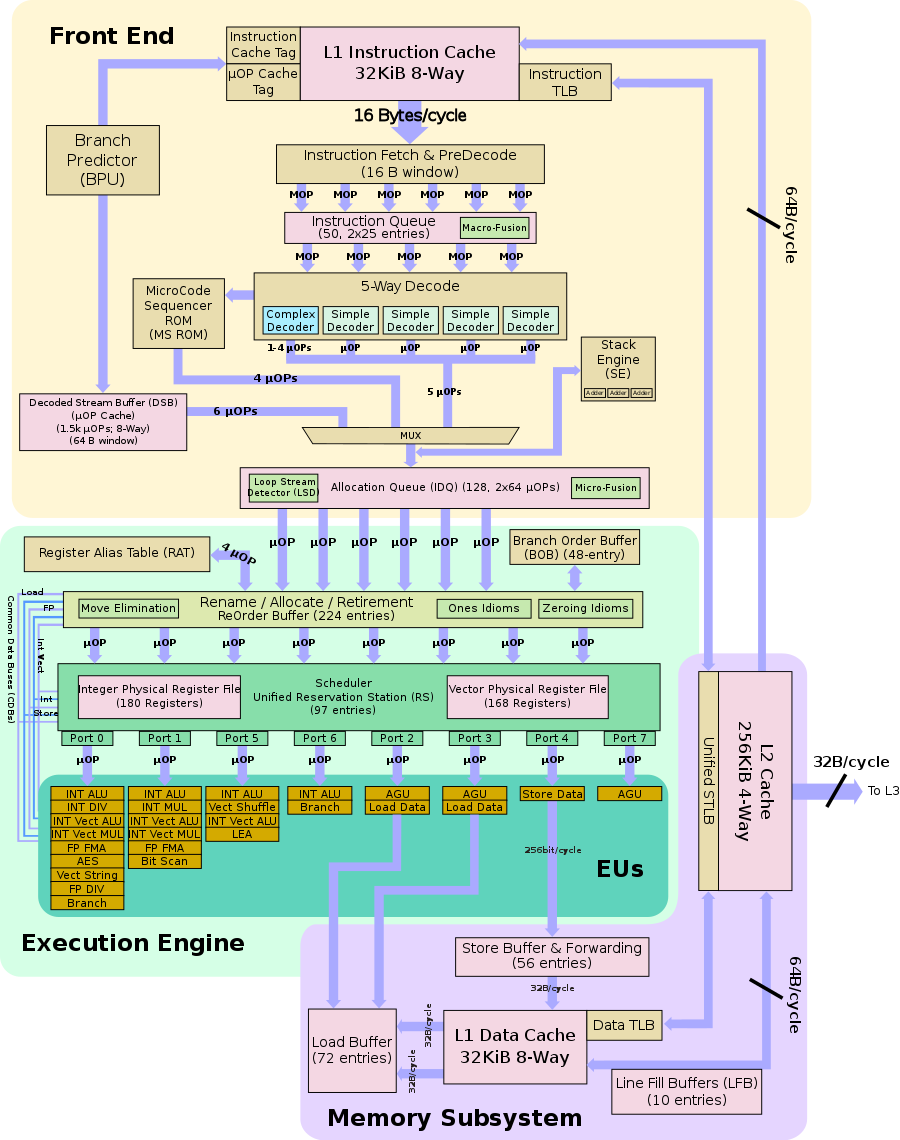
\includegraphics[width=0.94\textwidth]{./imgs/kaby.png}
      \end{center}
   \end{minipage}

   Για τον προσωπικό μου υπολογιστή, ο επεξεργαστής του Intel Core 
   \textbf{i7-8550U}
   χρησιμοποιεί την αρχιτεκτονική Kaby Lake.
   (https://en.wikichip.org/wiki/intel/microarchitectures/kaby\_lake).

   Όπως φαίνεται στο διάγραμμα, η αρχιτεκτονική Kaby Lake χρησιμοποιεί
   \textbf{ReOrder Buffer με 224 entries} (window size) και \textbf{Dispatch
   Width = 6 εντολές}. Σύμφωνα με την ανάλυση που προηγήθηκε, η επιλογή των
   χαρακτηριστικών αυτών είναι απολύτως λογική και δικαιολογητέα, αφού
   επιτυγχάνει αρκετά καλή απόδοση λαμβάνοντας υπ' όψιν το περιορισμένο μέγεθος
   chip και την χαμηλή κατανάλωση ενέργειας, εφόσον μάλιστα πρόκειται για
   επεξεργαστή προορισμένο για χρήση σε laptop. 
